\chapter{基于接收信号强度的几何模型发射源定位算法}
\label{cha:transmitter}

本章将要介绍基于接收信号强度的几何模型发射源定位算法,即用户作为信号发射源时实现对用户定位的算法。具体应用场景可以描述为:一个用户终端以恒定功率发射信号(比如蜂窝网或WLAN中用户上行通信),通信范围内的多个WAP(基站或是无线路由器)接收到信号并测得RSS,最后根据这些RSS实现对用户定位。

\section{路径损耗模型和估计器}

\subsection{路径损耗模型}

不妨设总共有$N$个WAP即信号接收者,则第$i$个接收者的RSS可用下式表示~\cite{erceg1999empirically}:
\begin{equation}
{P_i} = C - 10\alpha {\log _{10}}({\left\| {{\bm{\theta}} - {{\bm{\mathrm{x}}_i}}} \right\|_2}) + {n_i}, i = 1,2,...,N,\label{eq:rss}
\end{equation}
其中$P_i$是接收者的RSS,$\bm{\theta}$是发射源即用户的位置,$\alpha$是路径损耗系数,$C$是一个与$\bm{\theta}$ 和 $\bm{\mathrm{x}}_i$无关的常数,$n_i$则是均值为$0$、方差为${\sigma_i}^2$的高斯白噪声。为了简化表达,我们用下式代表发射源与第$i$个接收端之间的距离:
\begin{equation}
d_i = {\left\| {{\bm{\theta}} - {{\bm{\mathrm{x}}_i}}} \right\|_2}, \forall i. \label{eq:d}
\end{equation}
因为$C$是常数,所以它可以通过与另一个接收者的RSS相减被消除,即:
\begin{equation}
{P_{ij}} = 10\alpha ({\log _{10}}d_j - {\log _{10}}d_i) + {n_{ij}}, i \neq j, \label{eq:diff_rss}
\end{equation}
其中$P_{ij} = P_i - P_j$,$n_{ij}$变为$0$均值、方差为$\sigma_i^2 + \sigma_j^2$的高斯白噪声。注意到,因为我们没有锚点,这里我们取$i$作为RSS最大的接收者的下标。为了使表达更清晰,在接下来的部分我们将用$\bm{\mathrm{x}}_M, d_M$代表$\bm{\mathrm{x}}_i, d_i$。

\subsection{传统最大似然估计器}

传统最大似然(Maximum Likelihood, ML)估计器通过求解如下优化问题从而找到定位$\bm{\hat{\theta}}$:
\begin{equation}
\widehat {\bm{\theta }} = \mathop {\arg \min }\limits_{\bm{\theta }} \sum\limits_{j = 1}^N {{{[{P_{Mj}} - 10\alpha ({{\log }_{10}}d_j - {{\log }_{10}}d_M)]}^2}}, j \neq M. \label{eq:ml}
\end{equation}
因为这是一个非凸优化问题,许多凸优化估计器(比如半正定规划)和线性最小二乘估计被提出,正如第\ref{cha:intro}章所述。因为ML估计器是作为算法比较基准线的,我们需要选择一个能够取得最小误差的算法作为基准,因此我们直接优化最大似然函数。为了尽可能找到最优解,我们会多次随机初始点,选择损失函数最小的作为最终定位。

\subsection{基于几何的模型}

S. Wang 和 R. Inkol~\cite{wang2011near} 提出了一种线性最小二乘估计器(Linear Least Square, LLS),在推导过程中发现每两个接收端的RSS进行运算后可以形成一个发射源坐落在其上的圆。但是这个结论没有被作者直接用来优化,而是提出了两种线性最小二乘法。接下来我们将用这个知识得到基于几何的定位模型(Geometry-Based Model, GBM)。

如果我们忽略\eqref{eq:diff_rss}中的噪声项,可以得到:
\begin{equation}
{P_{ij}} - 5\alpha {\log _{10}}({\dfrac{d_j}{d_i}})^2 = 0, i \neq j. \label{eq:ignore}
\end{equation}
令:
\begin{equation}
\gamma = 10^{\frac{P_{ij}}{5\alpha}}, \label{eq:gamma}
\end{equation}
则\eqref{eq:ignore}可以被改写为:
\begin{equation}
{\left\| {\bm{\theta}  - \bm{\mathrm{x}}_j} \right\|_2}^2 = {\gamma _{ij}}{\left\| {\bm{\theta}  - \bm{\mathrm{x}}_i} \right\|_2}^2. \label{eq:10exp}
\end{equation}
如果 $\gamma _{ij} \neq 1$,即两个接收端的RSS不相等,\eqref{eq:10exp}可以被改写为:
\begin{equation}
{\left\| {\bm{\theta}  - \frac{\bm{\mathrm{x}}_j - \gamma_{ij}\bm{\mathrm{x}}_i}{1 - \gamma_{ij}}} \right\|_2}^2 = \frac{\gamma_{ij}{d_{ij}}^2}{(1 - \gamma_{ij})^2}, \label{eq:circle}
\end{equation}
其中$d_{ij} = \left\| \bm{\mathrm{x}}_i  - \bm{\mathrm{x}}_j \right\|_2$。显然这是一个$\bm{\theta}$坐落在其边缘上的圆,而圆心和半径分别为:
\begin{equation}
\bm{\mathrm{o}}_j = \frac{\bm{\mathrm{x}}_j - \gamma_{ij}\bm{\mathrm{x}}_i}{1 - \gamma_{ij}}, {r_j}^2 = \frac{\gamma_{ij}{d_{ij}}^2}{(1 - \gamma_{ij})^2}. \label{eq:oR}
\end{equation}

让$i$作为最大RSS接收端的下标(如果有多于1个最大RSS,则随机挑选一个而剔除其余的)并用$M$替换$i$。假设\eqref{eq:circle}被下面的加性噪声影响:
\begin{equation}
{\left\| {\bm{\theta}  - o_j} \right\|_2}^2 = d_j + n_j, j \neq M, \label{eq:GBMnoise}
\end{equation}
其中$n_j$是一个服从均值为$0$、方差为$\sigma_j^2$的截断高斯分布的噪声。因为$\bm{\theta}$是实数,因此\eqref{eq:GBMnoise}等式右边必须大于等于$0$,即$n_j$的取值范围是 $[-d_j, +\infty)$。所以我们建立了一个带有噪声$n_j$的模型,服从截断高斯分布。注意到这里的$n_j$与\eqref{eq:rss}中的噪声无关,因为这是两个独立的模型。

利用上述模型,我们可以定义一个服从截断高斯分布的随机变量$X_j = \left\|{\bm\theta} - \bm{\mathrm{o}}_j\right\|_2$,其概率密度函数是:
\begin{equation}
f(x_j) = \frac{1}{C(r_j)}\exp(-\frac{(x_j - r_j)^2}{2{\sigma_j}^2})I[0, +\infty), \label{eq:pdf}
\end{equation}
其中 $C(r_j) = \int_0^{ + \infty }\exp(-\frac{(x_j - r_j)^2}{2{\sigma_j}^2})dx_j$是归一化系数,$I[0, +\infty)$是指示函数,在$[0, +\infty)$范围内取值$1$否则为$0$。

因此,最终的损失函数和优化问题可以表示为:
\begin{equation}
\widehat {\bm{\theta }} = \mathop {\arg \min }\limits_{\bm{\theta }} \frac{1}{2}\sum\limits_{j = 1}^{N^-} {\frac{1}{\sigma_j^2}(\left\|{\bm\theta} - \bm{\mathrm{o}}_j\right\|_2 - r_j)^2}, \label{eq:loss}
\end{equation}
其中$N^-$代表剩余的接收端数量。因为$C(r_j)$和$\bm\theta$无关,因此在优化时可以忽略。

当假设所有接收端的噪声方差$\sigma_j^2$相等时,该优化问题就变成找到一个点,使得它到所有圆边缘的距离之和最小。因此这个优化问题有着明晰的几何意义,于是我们把\eqref{eq:loss}称为\textit{基于几何的模型(Geometry-Based Model, GBM)}。

因为无法证明GBM的凸性,我们将采用和ML中相同的方法求解,即多次随机挑选初始点后选取使得损失函数最小的结果。

后续的仿真结果表明GBM估计器是有偏的。但是注意到,我们的目标是最小化均方根误差(Mean Square Error, MSE)而MSE可以写作:
\begin{equation}    \label{eq:mse}
\begin{split}
MSE &= \mathrm{E}[(\widehat{\theta} - \theta)^2]\\
&= (\mathrm{E}[\widehat{\theta}] - \theta)^2 + \mathrm{E}[(\widehat{\theta} - \mathrm{E}[\widehat{\theta}])^2]\\
&= bias^2 + variance.
\end{split}
\end{equation}
即MSE是由估计器的偏差的平方和方差两部分组成,这也是机器学习领域经常出现的经典问题。若一个估计器有很小的偏差却有很大的方差则被称为“过拟合”(Over-Fitting)。在仿真和实测数据验证部分,我们发现传统最大似然估计器相比于GBM是过拟合的。

\section{克拉美罗下界(Cram\'{e}r-Rao Lower Bound, CRLB)}

CRLB是估计器的理论误差下界,虽然不一定能够达到,但是对其进行分析有助于研究估计器的性能。

\subsection{无偏估计的CRLB}

对于路径损耗模型,因为第$i$个接收端的RSS的分布服从$p_i \sim \mathcal{N}(-10\alpha\mathrm{log}_{10}{d_i} -C, {\sigma_i}^2)$,因此费舍信息(Fisher Information)可表示为:
\begin{equation}
I(\bm{\theta}) = (\frac{10\alpha}{\sigma\mathrm{ln}10})^2\sum\limits_{i = 1}^N(\frac{{\bm\theta} - \bm{\mathrm{x}}_i}{{\left\|{\bm\theta} - \bm{\mathrm{x}}_i\right\|_2}^2})(\frac{{\bm\theta} - \bm{\mathrm{x}}_i}{{\left\|{\bm\theta} - \bm{\mathrm{x}}_i\right\|_2}^2})^T, \label{eq:fisher}
\end{equation}
其中$\sigma$是噪声的标准差。如果估计器是无偏的,则协方差矩阵的CRLB为:
\begin{equation}
\begin{split}
CRLB(\bm{\theta}) &= I(\bm{\theta})^{-1} \label{eq:unbias_cov}\\
&\le Cov(\widehat{\bm{\theta}}_{ML}).
\end{split}
\end{equation}

因为最大似然估计器是渐进无偏的~ \cite{kay1993fundamentals},根据\eqref{eq:mse},最大似然法的RSME的估计下界可以表示为:
\begin{equation}
RMSE \ge \sqrt{Tr(CRLB)},\label{eq:rmse_ml}
\end{equation}
其中$Tr(\cdot)$是矩阵的迹,即对角线元素累加。

\subsection{有偏估计的CRLB}

假设GBM估计器的期望是$\bm\phi(\bm{\theta})$,如果估计器有偏,则协方差矩阵的CRLB可由下式所得:
\begin{equation}
\begin{split}
CRLB_{GBM}(\bm{\theta}) &= {\frac{\partial\bm\phi(\bm{\theta})}{\partial \bm\theta}}I(\bm{\theta})^{-1}{\frac{\partial\bm\phi(\bm{\theta})}{\partial \bm\theta}}^T\\
& \le Cov(\widehat{\bm{\theta}}_{GBM}),
\end{split}
\end{equation}
其中$\frac{\partial\bm\phi(\bm{\theta})}{\partial \bm\theta}$是雅可比(Jacobian)矩阵。注意到如果估计器是无偏的,则$\bm\phi(\bm{\theta}) = \bm{\theta}$即$\frac{\partial\bm\phi(\bm{\theta})}{\partial \bm\theta} = \bm{I}$,而这与\eqref{eq:unbias_cov}一致。

根据\eqref{eq:mse},GBM的RMSE的下界可表示为:
\begin{equation}
RMSE\! \ge\! \sqrt{{(\bm\phi(\bm{\theta})\! -\! \bm{\theta})}^T(\bm\phi(\bm{\theta})\! -\! \bm{\theta})\! +\! \mathrm{Tr}(CRLB_{GBM}(\bm{\theta}))}.\label{eq:rmse_gbm}
\end{equation}

直接计算$\bm\phi(\bm{\theta})$ 和 ${\frac{\partial\bm\phi(\bm{\theta})}{\partial \bm\theta}}$较困难,但是我们知道接收端RSS的分布,因此蒙特卡洛法适用于该问题。

首先,$\bm\phi(\bm{\theta})$比较容易用下式得到:
\begin{equation}
\begin{split}
\bm\phi(\bm{\theta}) &= \mathrm{E}[\widehat{\bm{\theta}}]\\
&\approx \frac{\sum\limits_{k = 1}^K{\widehat{\bm{\theta}}}}{K},
\end{split}
\end{equation}
其中,$K$是仿真次数。${\frac{\partial\bm\phi(\bm{\theta})}{\partial \bm\theta}}$可以直接用有限差分法得到,但是这可能需要大量时间计算,因为我们需要在二维平面内多次用不同的$\bm\theta$进行仿真。

接下来,我们将推导一种不需要用不同的$\bm\theta$仿真就可以得到${\frac{\partial\bm\phi(\bm{\theta})}{\partial \bm\theta}}$的方法。首先 $\bm\phi(\bm{\theta})$可以用如下公式表示:
\begin{equation}
\begin{split}
&Let \quad f(\bm{\theta}) = {\prod\limits_{i=1}^N}(2\pi{\sigma_i}^2)^{-\frac{1}{2}}e^{-\frac{(p_i + 10\alpha\mathrm{log}_{10}{d_i} + C)^2}{2{\sigma_i}^2}},\\
&then \quad \bm\phi(\bm{\theta}) = \iiint_{\mathbb{R}^N}\widehat{\bm{\theta}}f(\bm{\theta})dp_1...dp_N,
\end{split}
\end{equation}
其中$d_i$由\eqref{eq:d}定义。若$\widehat{\bm{\theta}}f(\bm{\theta})$ 和 $\frac{\partial \widehat{\bm{\theta}}f(\bm\theta)}{\partial \bm{\theta}}$是连续的,$\iiint_{\mathbb{R}^N}\widehat{\bm{\theta}}f(\bm\theta)$ 和 $\iiint_{\mathbb{R}^N}\frac{\partial \widehat{\bm{\theta}}f(\bm\theta)}{\partial \bm{\theta}}$一致收敛,则
\begin{equation}
\begin{split}
{\frac{\partial\bm\phi(\bm{\theta})}{\partial \bm\theta}} &= \frac{\partial\mathrm{E}[\widehat{\bm{\theta}}]}{\partial \bm{\theta}}\\
&= \frac{\partial}{\partial \bm{\theta}}\iiint_{\mathbb{R}^N} \widehat{\bm{\theta}}f(\bm{\theta}) dp_1...dp_N\\
&= \iiint_{\mathbb{R}^N} \frac{\partial \widehat{\bm{\theta}}f(\bm{\theta})}{\partial \bm{\theta}} dp_1...dp_N\\
&= \iiint_{\mathbb{R}^N} \sum\limits_{i=1}^N(p_i + 10\alpha\mathrm{log}_{10}{d_i} + C) \widehat{\bm{\theta}}(\frac{-10\alpha}{{\sigma_i}^2\mathrm{ln}10}\frac{{\bm\theta} - \bm{\mathrm{x}}_i}{{\left\|{\bm\theta} - \bm{\mathrm{x}}_i\right\|_2}^2})^Tf(\bm{\theta}) dp_1...dp_N\\
&= \mathrm{E}[\sum\limits_{i=1}^N(p_i + 10\alpha\mathrm{log}_{10}{d_i} + C)\widehat{\bm{\theta}}(\frac{-10\alpha}{{\sigma_i}^2\mathrm{ln}10}\frac{{\bm\theta} - \bm{\mathrm{x}}_i}{{\left\|{\bm\theta} - \bm{\mathrm{x}}_i\right\|_2}^2})^T]. \label{eq:mc}
\end{split}
\end{equation}
需要注意$\widehat{\bm{\theta}}$与$\bm{\theta}$无关,而是关于$(\bm{\mathrm{x}}_1,...,\bm{\mathrm{x}}_N)^T$ 和 $(P_1,...,P_N)^T$的函数。

根据\eqref{eq:mc}的结果,我们可以通过计算$\sum\limits_{i=1}^N(p_i + 10\alpha\mathrm{log}_{10}{d_i} + C)\widehat{\bm{\theta}}(\frac{-10\alpha}{{\sigma_i}^2\mathrm{ln}10}\frac{{\bm\theta} - \bm{\mathrm{x}}_i}{{\left\|{\bm\theta} - \bm{\mathrm{x}}_i\right\|_2}^2})^T$的经验平均值来利用蒙特卡洛法近似估算 ${\frac{\partial\bm\phi(\bm{\theta})}{\partial \bm\theta}}$,而不需要有限差分,这会大量节省仿真时间。

\section{RMSE的置信区间}

估计器的结果会受到噪声的影响,因此为了判断不同的估计器是否统计显著地不同,我们需要计算RMSE的置信区间(Confidence Interval)。

虽然RMSE的分布未知,但是幸运地,依据中心极限定理(Central Limit Theorem),当仿真次数很多且$({\widehat{\bm{\theta}}_k - \bm{\theta}})^T({\widehat{\bm{\theta}}_k - \bm{\theta}})$对于不同的$k$来说独立同分布,则MSE的分布将会趋近于正态分布,即
\begin{equation}
\begin{split}
\mathop{\mathrm{lim}}\limits_{K\rightarrow\infty}MSE &= \mathop{\mathrm{lim}}\limits_{K\rightarrow\infty} \frac{\sum\limits_{k=1}^K({\widehat{\bm{\theta}}_k - \bm{\theta}})^T({\widehat{\bm{\theta}}_k - \bm{\theta}})}{K} \\
&\sim \mathcal{N}(\mu, \frac{\sigma^2}{K}),
\end{split}
\end{equation}
其中$\mu$ 和 ${\sigma}^2$ 是 $({\widehat{\bm{\theta}}_k - \bm{\theta}})^T({\widehat{\bm{\theta}}_k - \bm{\theta}})$的期望和方差。因为我们不知道方差和期望,所以应当使用经验均值代替期望,即我们应当使用T检验。但是,在仿真次数足够多的情况下(在我们的场景下仿真了100,000次),我们可以直接使用Z检验。因此$95\%$置信区间可由下式获得:
\begin{equation}
CI = (\sqrt{RMSE^2 - 1.96\frac{\sigma}{\sqrt{K}}}, \sqrt{RMSE^2 + 1.96\frac{\sigma}{\sqrt{K}}}). \label{eq:ci}
\end{equation}
因此我们可以用\eqref{eq:ci}得到RMSE的置信区间并检验两个估计器的RMSE的差异是否具有统计显著性。

\section{数值仿真实验}

\subsection{仿真场景与估计器设置}

为了比较基于几何的模型(GBM),最大似然法(ML)以及线性最小二乘(LLS)估计器的定位效果,我们首先进行了仿真实验。仿真场景设置与S. Wang 和 R. Inkol~\cite{wang2011near} 的场景相同:发射源坐标为(0, 0),十个接收者的位置坐标为 (-126, 62), (-339, 166), (390, 76), (-178, 333), (482, 122), (-234, 141), (230, -45), (-352, 279), (-104, 465), (366, -139)。上述坐标的单位是米,分布如图\ref{fig:simscene}所示。在生成接收信号数据时,路径损耗系数$\alpha=4$,噪声服从0均值高斯分布,标准差从1变化到15,常数$C=-40$。

\begin{figure}[htb]
	\centering
	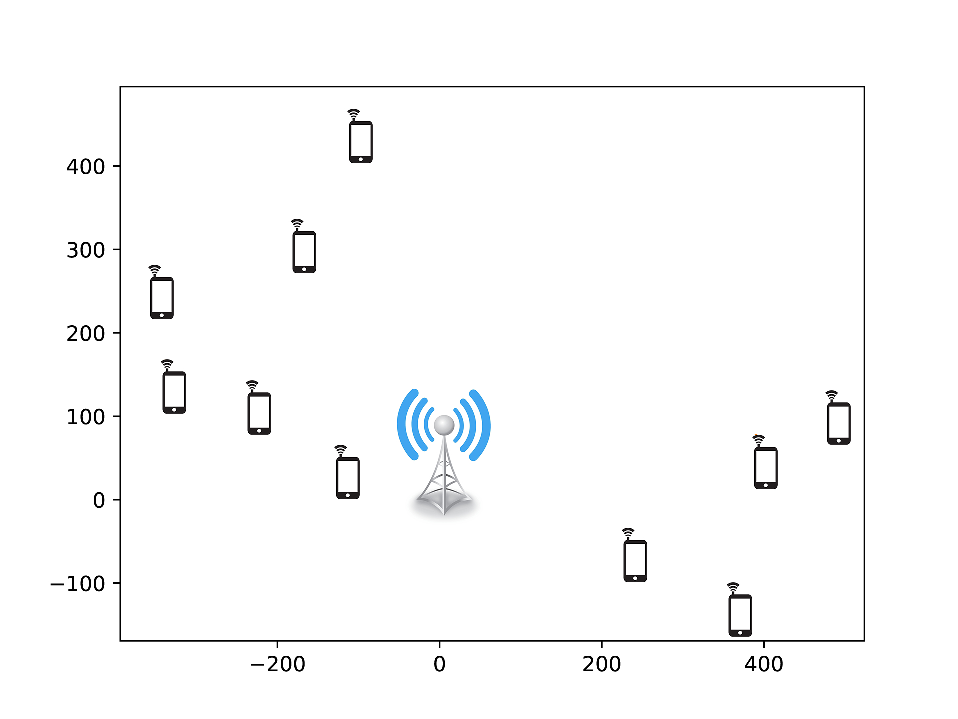
\includegraphics[width=\textwidth]{SimScene.pdf}
	\caption{仿真场景示意图,其中基站图标代表发射源位置,手机图标代表接收端位置。}
	\label{fig:simscene}
\end{figure}

因为GBM和ML都是非凸优化,因此我们将会以随机初始点进行20次迭代计算,使损失函数取得最小值的点作为最终定位点。初始点的二维坐标是从两个独立同分布的均匀分布$\mathcal{U}(-500, 500)$中采样所得。注意到我们的场景中没有锚点,因此必须选择一个接收端作为被减数,这里我们选择RSS最大的点。对于GBM,如果有多个最大值,则随机选择一个,其余的删除。GBM算法中的$\sigma_j$均被设为1。针对每个噪声方差,GBM、ML和LLS三种算法都仿真100,000次,之后计算RMSE及其置信区间。此外,无偏估计的CRLB以及GBM的CRLB分别根据\eqref{eq:rmse_ml}和\eqref{eq:rmse_gbm}计算。

\subsection{仿真结果}

\begin{figure}[htb]
	\centering
	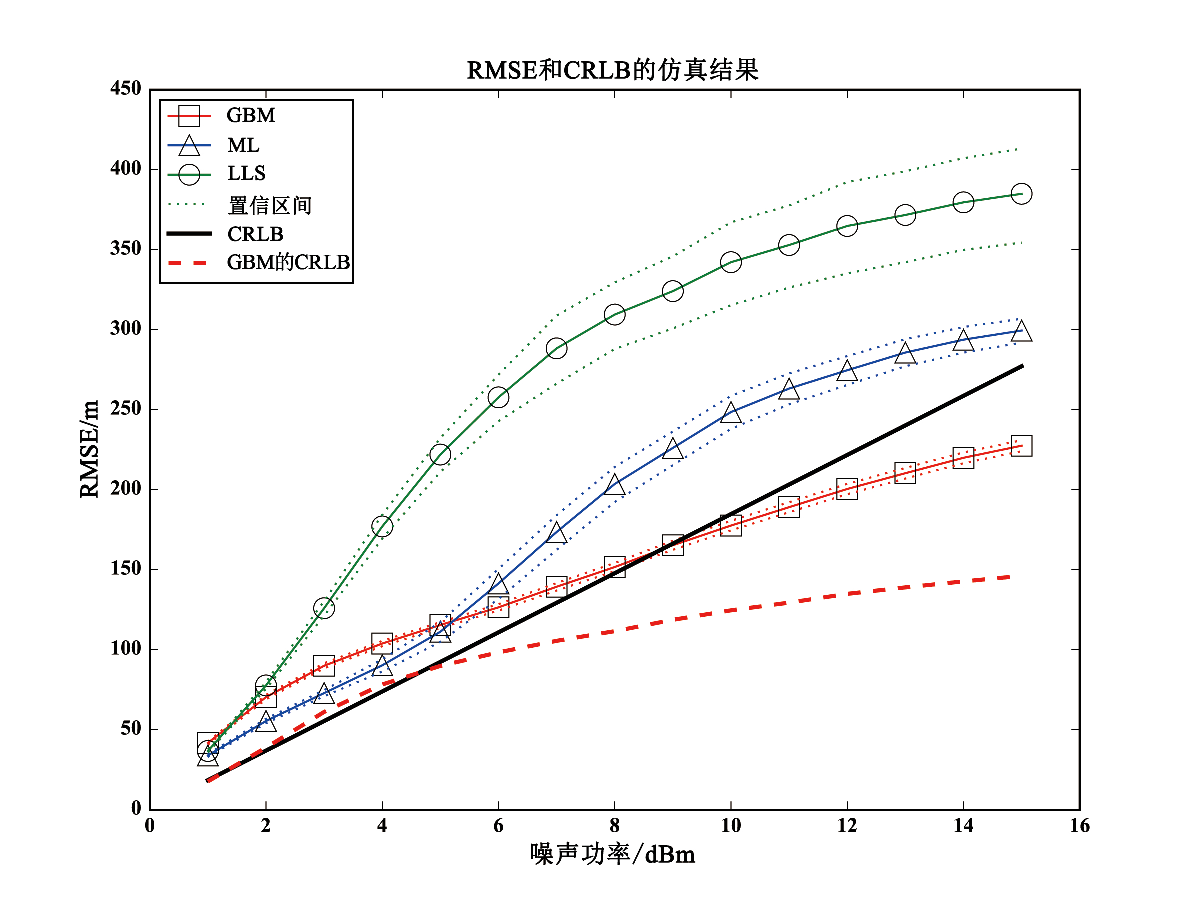
\includegraphics[width=\textwidth]{GBM_simulation.pdf}
	\caption{GBM、ML和LLS的RMSE、置信区间和CRLB的仿真结果。}
	\label{fig:gbm_sim}
\end{figure}

如图\ref{fig:gbm_sim}所示为100,000次仿真下,RMSE及其95\%置信区间和CRLB的结果。其中,正方形是我们的算法GBM的RMSE,上三角是ML的RMSE,圆圈是LLS的RMSE,点线为RMSE的95\%置信区间,实线是无偏估计的CRLB,虚线是通过蒙特卡洛法估计的GBM的CRLB。从仿真结果中可以看到,当噪声标准差$\sigma<5$dBm时ML的RMSE略低于GBM。然而当标准差$\sigma>5$dBm时,GBM的RMSE明显小于ML而且统计显著。因为多径效应和阴影效应的影响,真实世界场景中往往噪声功率较大。下一小节中,我们将上述三种算法用于实测数据,结果将为我们提供一些更深入的见解。除此之外,CRLB的结果和GBM与ML的情况相似。虽然GBM的CRLB比它的RMSE小得多,但是我们不知道是否存在一种估计器可以取得这个下界。这或许是下一步研究的可能突破点。

注意到,当噪声的标准差大于9之后,GBM的RMSE会比无偏估计的CRLB还低,这也暗示了GBM是有偏估计否则CRLB应是RMSE的下界。根据\eqref{eq:mse},虽然GBM是有偏估计,但是相比于方差的减小,偏置的稍微增加也不会使得总体MSE更大。从机器学习的角度来看,ML是一个低偏置、高方差的估计器,也就是说ML对于路径损耗模型“过拟合”了。而GBM类似于一种正则化版本,能够更好地适应高噪声数据。

最后,LLS估计器的RMSE最大。相比于LLS,ML能取得更小的RMSE已经被验证过~\cite{jackson2011received},而且当噪声较大时,LLS的性能会严重恶化~\cite{vaghefi2013cooperative}。我们的仿真结果与这些前人的结论一致。

\section{实测数据验证}

为了验证仿真结果并检测算法的在实际问题上的可用性,我们也采集了一些实测数据,根据接收信号强度对发射源定位。虽然我们算法设计的初衷是对用户定位,但是其实只要是信号发射源即可。因此为了数据采集的便利,我们的数据采集的是商用蜂窝网内基站的发射信号,车载路测仪作为接收端在道路上采集数据。

\subsection{数据介绍}

数据由车载路测仪在城市街道内运行采集移动通信基站的接收信号强度,其中共有超过120,000个基站。路测仪每5s采集一次GPS定位坐标、RSS、LAC (Location Area Code)、CID (Cell ID) 以及其他的基站信息。为了尽量最小化遮挡对信号衰减造成的影响,我们选择GSM(Global System for Mobile)信号用作测试。GSM的信号频段是900MHz和1.8GHz。

在定位之前,数据需要经过预处理。首先,将GPS的经纬度坐标转换为笛卡尔直角坐标系。其次,为了减少计算时间并降低阴影效应的影响,RSS$<-60$dBm的点将被删除。最后,满足如下要求的基站(发射源,目标定位点)将被选中进行实验:
\begin{itemize}
	\item 信号制式是GSM;
	\item 在基站的可接收范围内有至少10个接收点;
	\item 距离基站最近的接收点,其到基站的距离小于1000m。
\end{itemize}

经过筛选后,共有17,321个可用基站,这些数据将被用于实验。经过统计,这些基站的平均辐射半径为751m,即最小RSS对应的接收位置与基站之间的距离的平均值。后续的三个估计器的路径损耗系数$\alpha$均被设为4。

\subsection{实测数据实验结果}

\begin{table}[htb]
	\caption{实测数据实验结果}
	\begin{center}
		\begin{tabular}{cccc}
			\toprule
			\textbf{估计器} & \textbf{GBM} & \textbf{ML} & \textbf{LLS} \\
			\midrule
			\textbf{RMSE} [m] & 367.52 & 453.33 & 4898.10 \\
			\midrule
			\textbf{MAE}$^{a}$ [m] & 282.43 & 380.08 & 936.19 \\
			\bottomrule
			\multicolumn{3}{l}{$^{\mathrm{a}}$Mean Absolute Error.}
		\end{tabular}
		\label{tab:transmitter}
	\end{center}
\end{table}

表\ref{tab:transmitter}是实测数据的定位结果。相比于ML和LLS,GBM可以在RMSE和MAE(Mean Absolute Error,平均绝对值误差)上均取得更小的误差。其中MAE由下式计算:
\begin{equation}
MAE = \frac{\sum\limits_{k=1}^K{\left\| \widehat{\bm{\theta}} - \bm{\theta} \right\|}_2}{K}.
\end{equation}

根据仿真结果,当噪声较大时GBM的定位误差明显小于ML的事实,我们可以推测实测数据受噪声影响较大,因此GBM能取得小得多的定位误差。GBM的定位误差比ML的误差低将近100m,相对的,RMSE上降低了23.35\%,MAE上降低了34.75\%。从实验结果中我们可以发现,相比于ML,GBM更适用于在实际的商用无线网络中对发射源定位,因为真实环境噪声很大。此外,LLS的定位误差确认了前人工作中的论述,即LLS估计器的定位效果在噪声较大时会严重恶化。

\section{本章小结}

本章中,我们提出了一种基于接收信号强度的、利用几何模型对发射源定位的算法。除此之外,一种节省计算时间的、利用蒙特卡洛法估计GBM的RMSE的克拉美罗下界的方法也被提出,同时我们给出基于中心极限定理计算RMSE的置信区间的方法。仿真实验显示,相比于ML,在噪声方差较大时GBM算法可以取得明显更高的定位精度,即意味着GBM更加稳健。无偏估计的CRLB和GBM的CRLB呈现出和上述现象相似的结果。为了验证仿真结果并测试算法实用性,我们还从商用蜂窝网内采集数据进行测试。实验结果显示,GBM在RMSE和MAE上均取得更小的定位误差,相比于ML的RMSE和MAE分别降低了18.9\%和25.7\%。这个结果说明,当与ML对比时,GBM更适用于真实场景下的发射源定位需求。






